\section{Hàm số mũ - Hàm số Logarit}

\subsection{Đề 1}

\Opensolutionfile{ans}[ans/ans-K11-C6-B3-D1]
\caulc

\begin{ex}%[Thành Đạt - Dự án Tex hoá tài liệu Dương Hùng]%[1D6N3-1]
	Tập giá trị của hàm số $y=\mathrm{e}^{-2x+4}$ là
	\choice
	{\True$(0;+\infty)$}
	{$[0;+\infty)$}
	{$\mathbb{R}\setminus\{0\}$}
	{$\mathbb{R}$}
	\loigiai{
		Vì $\mathrm{e}^{-2x+4}>0\ \forall x\in\mathbb{R}$ nên tập giá trị của hàm số là $(0;+\infty)$.
	}
\end{ex}

\begin{ex}%[Thành Đạt - Dự án Tex hoá tài liệu Dương Hùng]%[1D6N3-2]
	Tập xác định của hàm số $y=\log_3 \left(2x+1\right)$ là
	\choice
	{$\left(-\infty;\dfrac{1}{2}\right)$}
	{ $\left(\dfrac{1}{2};+\infty\right)$}
	{$\left(0;+\infty\right)$}
	{\True $\left(-\dfrac{1}{2};+\infty\right)$}
	\loigiai
	{
		Hàm số $y=\log_3 \left(2x+1\right)$ xác định khi và chỉ khi $2x+1>0 \Leftrightarrow  x>-\dfrac{1}{2}$.\\
		Vậy tập xác định của hàm số là $\mathscr{D} = \left(-\dfrac{1}{2};+\infty\right)$.
	}
\end{ex}

\begin{ex}%[Thành Đạt - Dự án Tex hoá tài liệu Dương Hùng]%[1D6H3-2]
	Tìm tập xác định $\mathscr{D}$ của hàm số $y=(2x-x^2)^{\frac{1}{3}}+\log_2(x-1)^2$.
	\choice
	{$\mathscr{D}=(0;2)$}
	{$\mathscr{D}=(0;1)$}
	{$\mathscr{D}=\mathbb{R}\setminus \{0;2\}$}
	{\True $\mathscr{D}=(0;2)\setminus \{1\}$}
	\loigiai{
		Điều kiện: $\heva{&2x-x^2>0\\ &(x-1)^2>0}\Leftrightarrow \heva{&0<x<2\\ &x-1\neq 0}\Leftrightarrow \heva{&0<x<2\\&x\neq 1}$.\\
		Tập xác định $\mathscr{D}=(0;2)\setminus \{1\}$.\\
		\textbf{Cần nhớ: }$A^2>0 \Rightarrow A\neq 0$ và $|A|>0 \Leftrightarrow A\neq 0$.
	}
\end{ex}

\begin{ex}%[Thành Đạt - Dự án Tex hoá tài liệu Dương Hùng]%[1D6N3-2]
	Tập xác định của hàm số $y=4^x$ là
	\choice
	{$\mathbb{R}\setminus\{0\}$}
	{$[0;+\infty)$}
	{$(0;+\infty)$}
	{\True $\mathbb{R}$}
	\loigiai{
		Ta có hàm số mũ $y=4^x$	luôn xác định với mọi $x\in\mathbb{R}$.}
\end{ex}


\begin{ex}%[Thành Đạt - Dự án Tex hoá tài liệu Dương Hùng]%[1D6H3-2]
	Tập xác định của hàm số $y=\log_2 \left(x^2-2x-3\right)$ là
	\choice
	{$\left( -\infty ;-1 \right]\cup \left[ 3;+\infty  \right)$}
	{$\left[ -1;3 \right]$}
	{\True $\left( -\infty ;-1 \right)\cup \left( 3;+\infty  \right)$}
	{$\left( -1;3\right)$}
	\loigiai
	{
		Hàm số $y=\log_2 \left(x^2-2x-3\right)$ xác định khi và chỉ khi $x^2-2x-3>0 \Leftrightarrow \hoac{&x<-1\\&x>3}$.\\
		Vậy tập xác định của hàm số là $\mathscr{D} = \left( -\infty ;-1 \right)\cup \left( 3;+\infty  \right)$.
	}
\end{ex}

\begin{ex}%[Thành Đạt - Dự án Tex hoá tài liệu Dương Hùng]%[1D6H3-3]
	\immini{
		Tìm $a$ để hàm số $y=\log_a x$ $(0<a \ne 1)$ có đồ thị là hình bên.
		\choice
		{\True $a=\sqrt{2}$}
		{$a=\dfrac{1}{\sqrt{2}}$}
		{$a=\dfrac{1}{2}$}
		{$a=2$}
	}{
		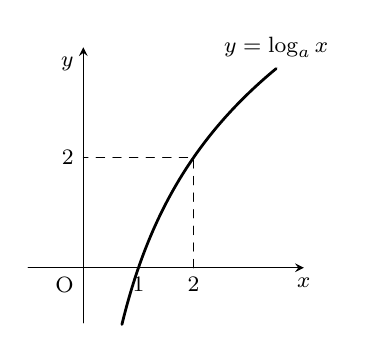
\begin{tikzpicture}[scale=0.7, font=\footnotesize, line join=round, line cap=round, >=stealth]
			\draw[->] (-1,0)--(0,0) node[below left]{O}--(4,0) node[below]{$x$};
			\draw[->] (0,-1)--(0,4) node[below left]{$y$};
			\draw[smooth, black, line width=1,samples=80] plot[domain=0.7:3.5] (\x,{2*log2(\x)}) node[above]{$y=\log_ax$};
			\draw[dashed] (1,0) node[below]{$1$} (2,0) node[below]{$2$} (0,2) node[left]{$2$};
			\draw[dashed] (2,0)--(2,2)--(0,2);
		\end{tikzpicture}
	}
	\loigiai{Đồ thị hàm số đi qua điểm $(2;2)$ nên  $2=\log_a 2 \Leftrightarrow a^2=2 \Leftrightarrow a=\sqrt{2}$.
	}
\end{ex}

\begin{ex}%[Thành Đạt - Dự án Tex hoá tài liệu Dương Hùng]%[1D6H3-3]
	\immini{
		Đường cong ở hình bên là đồ thị của hàm số nào
		\choice
		{$y=2^x$}
		{$y=\log_2 x$}
		{$y=\left(\dfrac{1}{2}\right)^x$}
		{\True $y=\log_{\frac{1}{2}} x$}
	}{
		\begin{tikzpicture}[>=stealth,scale=0.7, line join=round, line cap=round]
			\def\xmax{3} \def\ymin{-1} \def\ymax{2}
			%\draw[line width=0.1pt,dashed] (-0.9,\ymin) grid (\xmax,\ymax);
			\draw[->] (-0.5,0)--(\xmax,0) node [below]{$x$};
			\draw[->] (0,\ymin)--(0,\ymax) node [left]{$y$};
			\node at (0,0) [below left]{$O$};
			\clip (-0.9,\ymin) rectangle (\xmax-0.1,\ymax-0.1);
			\draw[smooth,samples=300,domain=0.3:2] plot(\x,{ln(\x)/ln(0.5)});
		\end{tikzpicture}
	}
	\loigiai
	{Quan sát hình dáng đồ thị ta thấy đồ thị nằm bên phải trục $Oy$, đồ thị đi xuống từ trái sang phải .
	}
\end{ex}

\begin{ex}%[Thành Đạt - Dự án Tex hoá tài liệu Dương Hùng]%[1D6H3-3]
	\immini
	{
		Cho hai hàm số $y=a^x$ và $y=\log_b x$ có đồ thị như hình vẽ. Mệnh đề nào sau đây là đúng.
		\choice
		{\True $a>1; 0<b<1$}
		{$0<a<1; 0<b<1$}
		{$0<a<1; b>1$}
		{$a>1; b>1$}
	}
	{
		\begin{tikzpicture}[>=stealth,scale=0.7, line join=round, line cap=round]
			\draw[->] (-2,0)--(4,0) node [below]{$x$};
			\draw[->] (0,-2)--(0,3) node [left]{$y$};
			\node at (0,0) [below right]{$O$};
			\clip (-3,-3) rectangle (4,4);
			\fill[black](0,1) circle (2pt) node[above left] {$1$} (1,0) circle (2pt) node [below] {$1$};
			\draw[smooth,samples=150,domain=-2:1.5] plot(\x,{2^(\x)});
			\draw[smooth,samples=150,domain=0.3:3] plot(\x,{-ln(\x)/ln(2)});
			\node at (2,2){$y=a^x$};
			\node at (1.7,-0.6)[right]{$y=\log_{b}x$};
		\end{tikzpicture}
	}
	\loigiai{
		Quan sát đồ thị ta thấy :\\
		Hàm số $y=a^x$ đồng biến nên $a>1$.\\
		Hàm số $y=\log_b x$ nghịch biến nên $0<b<1$.
	}
\end{ex}

\begin{ex}%[Thành Đạt - Dự án Tex hoá tài liệu Dương Hùng]%[1D6V3-2]
	Số giá trị nguyên của tham số $m \in(-2024 ; 2024)$ để hàm số $y=\left(x^{2}-2 x-m+1\right)^{\sqrt{5}}$ xác định với $\forall x \in \mathbb{R}$ là
	\choice
	{$4048$}
	{$2024$}
	{\True $2023$}
	{Vô số}
	\loigiai{
		Cần nhớ với $f(x)=a x^2 + b x + c$ ($a\ne 0$) thì $f(x) > 0$ với mọi $x\in\mathbb{R}$ khi và chỉ khi xảy ra một trong hai trường hợp:
		\begin{itemize}
			\item $a>0$ và $\Delta<0$;
			\item $a = 0$, $b=0$, $c>0$.
		\end{itemize}
		Hàm số xác định khi và chỉ khi $x^2 - 2x - m + 1>0$.\\
		Để $\mathscr{D}=\mathbb{R}$ thì $x^2 - 2x - m + 1>0$ luôn đúng với $\forall x\in\mathbb{R}$, điều này tương đương với 
		\[
			\heva{&a=1>0\\&\Delta=4 - 4(-m + 1)<0}\Leftrightarrow m<0.
		\]
		Kết hợp với $m\in\mathbb{Z}$ và $m \in ( - 2024 ; 2024)$ nên $m\in\{ - 2023 ;\ldots ; - 1\}$. \\
		Vậy có $2023$ số nguyên $m$ thoả mãn.
		
	}
\end{ex}

\begin{ex}%[Thành Đạt - Dự án Tex hoá tài liệu Dương Hùng]%[1D6H3-3]
	Tìm tất cả các giá trị của $a$ để hàm số $ y = ( 2 - a )^x $ nghịch biến trên $ \mathbb{R} $.
	\choice
	{$ 2 < a < 3 $}
	{\True $ 1 < a < 2 $}
	{$ a > 2 $}
	{$ 0 < a < 1 $}
	\loigiai{
		Hàm số $ y = (2 - a)^x $ nghịch biến trên $ \mathbb{R} \Leftrightarrow 0 < 2 - a < 1 \Leftrightarrow 1 < a < 2 $.
	}
\end{ex}

\begin{ex}%[Thành Đạt - Dự án Tex hoá tài liệu Dương Hùng]%[1D6V3-3]
	\immini
	{
		Cho ba hàm số $y=a^x,y=b^x, y=c^x$, với $a,b,c$ là hai số thực dương khác $1$ lần lượt có đồ thị như hình bên. Khẳng định nào sau đây đúng?
		\choice
		{$a<b<c$}
		{\True $a<c<b$}
		{$b<c<a$}
		{$c<a<b$}
	}
	{
		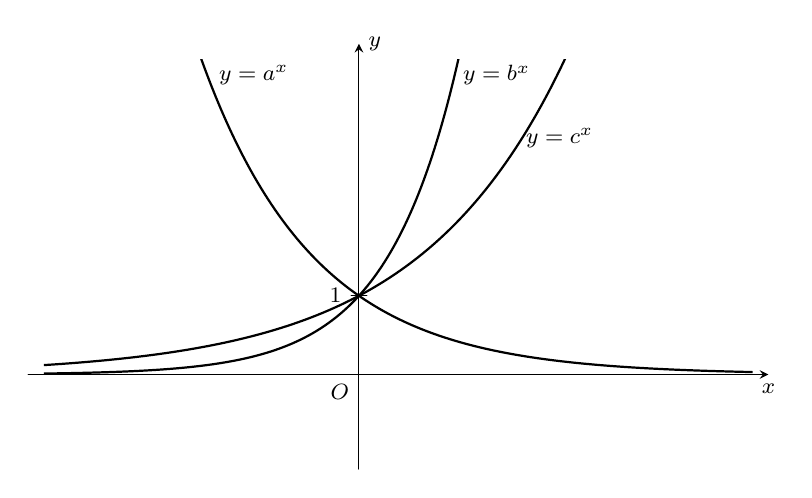
\begin{tikzpicture}[scale=1, font=\footnotesize, line join=round, line cap=round, >=stealth]
			\def\xmin{-4}\def\xmax{5}\def\ymin{-1}\def\ymax{4}
			\draw[->] (\xmin-0.2,0)--(\xmax+0.2,0) node[below] {\footnotesize $x$};
			\draw[->] (0,\ymin-0.2)--(0,\ymax+0.2) node[right] {\footnotesize $y$};
			\draw (0,0) node [below left] {\footnotesize $O$};
			\foreach \x in {}\draw (\x,0.1)--(\x,-0.1) node [below] {\footnotesize $\x$};
			\foreach \y in {1}\draw (0.1,\y)--(-0.1,\y) node [left] {\footnotesize $\y$};
			\clip (\xmin,\ymin) rectangle (\xmax,\ymax);
			\draw[thick,smooth,samples=200,domain=\xmin:\xmax] plot (\x,{3^\x});
			\draw (1.2,3.8) node [right]{$y=b^x$};
			\draw[thick,smooth,samples=200,domain=\xmin:\xmax] plot (\x,{.5^\x});
			\draw (-1.9,3.8) node [right]{$y=a^x$};
			\draw[thick,smooth,samples=200,domain=\xmin:\xmax] plot (\x,{1.7^\x});
			\draw (2,3) node [right]{$y=c^x$};
		\end{tikzpicture}
	}
	
	\loigiai
	{\immini{	Kẻ đường thẳng $x=1$ cắt các đồ thị hàm số tại các điểm lần lượt có tung độ là $a,c,b$ như hình trên.
			Từ đồ thị ta có
			\[
				0<a<1<c<b.
			\]
		}
		{
			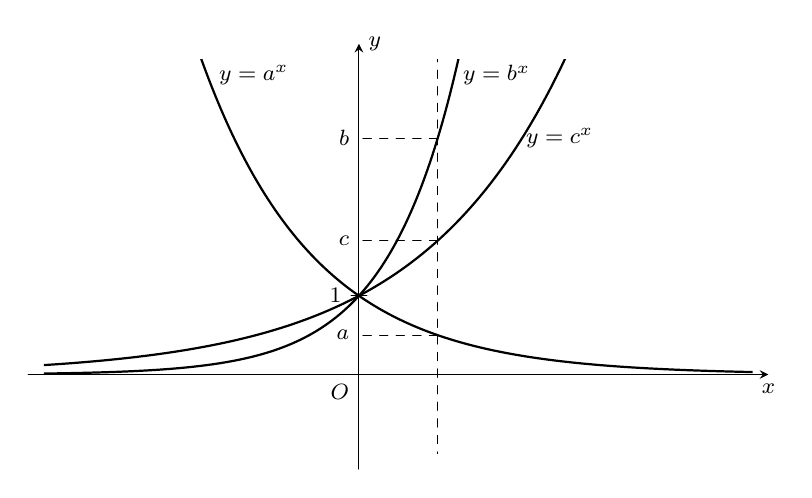
\begin{tikzpicture}[scale=1, font=\footnotesize, line join=round, line cap=round, >=stealth]
				\def\xmin{-4}\def\xmax{5}\def\ymin{-1}\def\ymax{4}
				\draw[->] (\xmin-0.2,0)--(\xmax+0.2,0) node[below] {\footnotesize $x$};
				\draw[->] (0,\ymin-0.2)--(0,\ymax+0.2) node[right] {\footnotesize $y$};
				\draw (0,0) node [below left] {\footnotesize $O$};
				\foreach \x in {}\draw (\x,0.1)--(\x,-0.1) node [below] {\footnotesize $\x$};
				\foreach \y in {1}\draw (0.1,\y)--(-0.1,\y) node [left] {\footnotesize $\y$};
				\clip (\xmin,\ymin) rectangle (\xmax,\ymax);
				\draw[thick,smooth,samples=200,domain=\xmin:\xmax] plot (\x,{3^\x});
				\draw (1.2,3.8) node [right]{$y=b^x$};
				\draw[thick,smooth,samples=200,domain=\xmin:\xmax] plot (\x,{.5^\x});
				\draw (-1.9,3.8) node [right]{$y=a^x$};
				\draw[thick,smooth,samples=200,domain=\xmin:\xmax] plot (\x,{1.7^\x});
				\draw (2,3) node [right]{$y=c^x$};
				\draw[dashed] (1,-1.3)node[below]{$1$}--(1,4.1) (1,3)--(0,3) node[left]{$b$} (1,.5)--(0,.5) node[left]{$a$} (1,1.7)--(0,1.7) node[left]{$c$};
			\end{tikzpicture}
		}
		
	}
\end{ex}

\begin{ex}%[Thành Đạt - Dự án Tex hoá tài liệu Dương Hùng]%[1D6V3-3]
	Biết đồ thị của hàm số $y=f\left(x\right)$ đối xứng với đồ thị hàm số $y=\log_ax \, \left(0<a\ne 1\right)$ qua điểm $I\left(2;2\right)$. Giá trị của $f\left(4-a^{2018}\right)$ là
	\choice
	{$-2020$}
	{$2014$}
	{\True $-2014$}
	{$2020$}
	\loigiai
	{
		Gọi $M\left(x;\log_ax\right)$ là điểm thuộc đồ thị hàm số $y=\log_ax$ thì điểm đối xứng với $M$ qua $I$ là ${M}'\left(4-x;4-\log_ax\right)$ thuộc đồ thị hàm số $y=f(x)$.\\
		Do đó $f\left(4-x\right)=4-\log_ax$.
		Suy ra: $f\left(4-a^{2018}\right)=4-\log_aa^{2018}=-2014$
	}
\end{ex}

\Closesolutionfile{ans}
\indapan{6}{ans/ans-K11-C6-B3-D1}
\cauds
\Opensolutionfile{ans}[ans/ans-K11-C6-B3-D1-DS]

\begin{ex}%[Thành Đạt - Dự án Tex hoá tài liệu Dương Hùng]%[1D6H3-2]
	Tìm tập xác định của các hàm số.
	\choiceTF
%	[t]
	{\True Hàm số $y=2^x$ có tập xác định là $\mathscr{D} = \mathbb{R}$}
	{\True Hàm số $y = \left( \dfrac{1}{3} \right)^x + 2\mathrm{e}^x$ có tập xác định $\mathscr{D} = \mathbb{R}$}
	{Hàm số $y = \log_2 (x-x^2)$ có tập xác định là $\mathscr{D} = \left[ 0;\dfrac{1}{3} \right]$}
	{Hàm số $y = \ln x^2 + 3\log(x+2)$ có tập xác định là $\mathscr{D} = (-2;+\infty)$}
	\loigiai{
		\begin{itemchoice}
			\itemch \textbf{Đúng}. 
			\itemch \textbf{Đúng}.
			\itemch \textbf{Sai}. Vì hàm số xác định khi $x-x^2 > 0 \Leftrightarrow 0 < x < \dfrac{1}{3}$.
			\itemch \textbf{Sai}. Vì hàm số xác định khi $\heva{&x^2 > 0\\ &x+2>0} \Leftrightarrow \heva{&x>-2\\ &x\ne 0.}$ 
		\end{itemchoice}	
	}
\end{ex}

\begin{ex}%[Thành Đạt - Dự án Tex hoá tài liệu Dương Hùng]%[1D6H3-3]
	Cho hàm số $y=3^x$ có đồ thị $(C)$.
	\choiceTF
%	[t]
	{\True Tập xác định của hàm số là $\mathscr{D} = \mathbb{R}$}
	{Hàm số nghịch biến trên $(0;2)$}
	{$A(2;6)$ thuộc $(C)$}
	{\True $(C)$ nằm hoàn toàn trên trục hoành}
	\loigiai{
		\begin{itemchoice}
			\itemch \textbf{Đúng}. 
			\itemch \textbf{Sai}. Do $3>1$ nên hàm số luôn đồng biến trên $\mathbb{R}$.
			\itemch \textbf{Sai}. Vì $x=2$ thì $y=9$ nên $A(2;6)\notin (C)$.
			\itemch \textbf{Đúng}. 
		\end{itemchoice}	
	}
\end{ex}

\begin{ex}%[Thành Đạt - Dự án Tex hoá tài liệu Dương Hùng]%[1D6H3-3]
	Xét sự biến thiên của các hàm số.
	\choiceTF
%	[t]
	{\True Hàm số $y = \left(\dfrac{\sqrt{2} + \sqrt{3}}{2}\right)^x$ đồng biến trên $\mathbb{R}$}
	{\True Hàm số $y=\log_2 x$ đồng biến trên $(0;+\infty)$}
	{Hàm số $\left(\dfrac{\pi}{\mathrm{e}}\right)^x$ nghịch biến trên $\mathbb{R}$}
	{Hàm số $y = \dfrac{1}{\log x}$ đồng biến trên $\mathbb{R}$}
	\loigiai{
		\begin{itemchoice}
			\itemch \textbf{Đúng}. Vì $\dfrac{\sqrt{2} + \sqrt{3}}{2} > 1$. 
			\itemch \textbf{Đúng}. Vì $2>1$.
			\itemch \textbf{Sai}. Vì $\dfrac{\pi}{\mathrm{e}} < 1$.
			\itemch \textbf{Sai}. Vì $\log \dfrac{1}{x} = \log_{0{,}1} x$ và $0< 0{,}1 < 1$ nên hàm số $y=\log \dfrac{1}{x}$ nghịch biến trên $(0;+\infty)$. 
		\end{itemchoice}	
	}
\end{ex}

\begin{ex}%[Thành Đạt - Dự án Tex hoá tài liệu Dương Hùng]%[1D6H3-4]
	Cho $a$, $b$ là các số thực.
	\choiceTF
%	[t]
	{\True $a >1$ nên $a^{\sqrt{2}} < a^{\sqrt{3}}$}
	{$0<a<1$ nên $\log_a 30 > \log_a 29{,}7$}
	{$0 < b < 1$ nên $b^{\tfrac{\sqrt{3}}{4}} < b^{\tfrac{\sqrt{2}}{3}}$}
	{\True $b>1$ nên $\log_b 7 > \log_b 2$}
	\loigiai{
		\begin{itemchoice}
			\itemch \textbf{Đúng}. Vì $a>1$ nên hàm số $y=a^x$ đồng biến trên $\mathbb{R}$ và $\sqrt{2} < \sqrt{3}$ nên $a^{\sqrt{2}} < a^{\sqrt{3}}$.  
			\itemch \textbf{Sai}. Vì $0<a<1$ nên hàm số $y = \log_a x$ nghịch biến trên $(0;+\infty)$ và $30 > 29{,}7$ nên $\log_a 30 < \log_a 29{,}7$.
			\itemch \textbf{Sai}. Vì $0<b<1$ nên hàm số $y=b^x$ nghịch biến trên $\mathbb{R}$ và $\dfrac{\sqrt{3}}{4} < \dfrac{\sqrt{2}}{3}$ nên $b^{\tfrac{\sqrt{3}}{4}} > b^{\tfrac{\sqrt{2}}{3}}$.
			\itemch \textbf{Đúng}. Vì $b>1$ nên hàm số $y = \log_b x$ đồng biến trên $(0;+\infty)$ và $7 > 2$ nên $\log_b 7 > \log_b 2$.
		\end{itemchoice}	
	}
\end{ex}

\Closesolutionfile{ans}
\indapan{3}{ans/ans-K11-C6-B3-D1-DS}

\Opensolutionfile{ans}[ans/ans-K11-C6-B3-D1-KQ]
\caukq

\begin{ex}%[Thành Đạt - Dự án Tex hoá tài liệu Dương Hùng]%[1D6H3-3]
	Cho đồ thị của hàm số $y=\log_2(ax+b)$ đi qua điểm $A(1;3)$ và $B(9;6)$. Tính giá trị $a+3b$.
	\shortans{$10$}
	\loigiai{
		Ta có $\heva{&\log_2(a+b) = 3\\ &\log_2(9a+b) = 6} \Leftrightarrow \heva{&a+b=8\\ &9a+b=64} \Leftrightarrow\heva{&a=7\\ &b=1.}$\\
		Vậy $a+3b=10$.
	}
\end{ex}

\begin{ex}%[Thành Đạt - Dự án Tex hoá tài liệu Dương Hùng]%[1D6H3-2]
	Tập xác định của hàm số $y = (9-x^2)^{\sqrt{3}} + \log (x-1)$ là $(a;b)$ với $a$, $b$ là các số nguyên. Tính giá trị $a+b$.
	\shortans{$4$}
	\loigiai{
		Hàm số xác định khi và chỉ khi $\heva{&9-x^2 >0\\ &x-1>0} \Leftrightarrow \heva{&-3 < x <3\\ &x>1} \Leftrightarrow1 < x < 3$.\\
		Vậy $a=1$, $b=3$ nên $a+b=4$.
	}
\end{ex}

\begin{ex}%[Thành Đạt - Dự án Tex hoá tài liệu Dương Hùng]%[1D6H3-2]
	Biết $\mathscr{D}=(a;b)$ là tập xác định của hàm số $y=(2-x)^{e}+\log_2 x$. Tính giá trị $a+b$.
	\shortans{$2$}
	\loigiai{
		Hàm số xác định khi $\heva{& 2-x>0 \\ &x>0}\Leftrightarrow 0 < x < 2$.\\
		Vậy $a+b=2$.
	}
\end{ex}

\begin{ex}%[Thành Đạt - Dự án Tex hoá tài liệu Dương Hùng]%[1D6C3-2]
	Tìm số giá trị nguyên âm của tham số $m$ để hàm số $y=\ln \left(x+\dfrac{1}{x-1}+m\right)$ xác định với mọi $x$ thuộc khoảng $\left(1;+\infty\right)$.
	\shortans{$2$}
	\loigiai{
		Từ giả thiết suy ra $x+\dfrac{1}{x-1}+m>0$ với mọi $x\in\left(1;+\infty\right)$.\\
		Suy ra $x+\dfrac{1}{x-1}>-m$ với mọi $x\in \left(1;+\infty\right)$.\\
		Theo bất đẳng thức Cô-si ta có $x+\dfrac{1}{x-1}=x-1+\dfrac{1}{x-1}+1\ge 3$ với $x>1$.\\
		Dấu bằng xảy ra khi $x-1=\dfrac{1}{x-1}\Rightarrow x=2$ (thỏa mãn).\\
		Từ đó $3>-m\Leftrightarrow m>-3$, mà $m$ nguyên âm nên $m\in\{-2;-1\}$.
	}
\end{ex}

\begin{ex}%[Thành Đạt - Dự án Tex hoá tài liệu Dương Hùng]%[1D6V3-2]
	Cho hàm số $y = \ln \left( x^2 -2x -m+1 \right)$ với $m$ là tham số thực. Tìm số giá trị nguyên dương của $m$ để hàm số xác định trên $[5;10]$. 
	\shortans{$15$}
	\loigiai{
		Hàm số $y=\ln\left(x^2 -2x -m+1\right)$ xác định trên $[1;3]$ khi và chỉ khi
		\[
			x^2 - 2x - m + 1 > 0, \forall x\in[5;10] \Leftrightarrow m < (x-1)^2,\forall x\in[5;10]
			\Leftrightarrow m < \min\limits_{[5;10]} (x-1)^2 = 16.
 		\]
 		Kết hợp với $m$ nguyên dương ta thu được $15$ giá trị của $m$ thoả mãn.
	}
\end{ex}

\begin{ex}%[Thành Đạt - Dự án Tex hoá tài liệu Dương Hùng]%[1D6V3-5]
	Trong một phòng thí nghiệm, người ta nuôi một loại vi khuẩn. Ban đầu có $300$ vi khuẩn và sau $1$ giờ thì số vi khuẩn là $705$ con. Giả sử số vi khuẩn tại thời điểm $x$ (giờ) được tính theo hàm mũ là $f(x) = C\mathrm{e}^{kx}$ với $C$ và $k$ là các hằng số thực dương. Xác định số vi khuẩn sau $5$ giờ tính theo đơn vị nghìn con (kết quả lấy $1$ chữ số sau dấu thập phân).
	\shortans{$21{,}5$}
	\loigiai{
		Ta có $300 = f(0) = C$ và $705 = f(1) = C\mathrm{e}^k = 300\mathrm{e}^k$ nên $\mathrm{e}^k = \dfrac{705}{300} = 2{,}35$ hay $f(x) = 300\cdot (2{,}35)^x$.\\
		Do đó $f(5) = 300\cdot (2{,}35)^5 \approx 21501 \approx 21{,}5$ nghìn con. 
	}
\end{ex}


\Closesolutionfile{ans}
\indapan{6}{ans/ans-K11-C6-B3-D1-KQ}


\subsection{Đề 2}

\Opensolutionfile{ans}[ans/ans-K11-C6-B3-D2]
\caulc

\begin{ex}%[Thành Đạt - Dự án Tex hoá tài liệu Dương Hùng]%[1D6N3-2]
	Tìm tập xác định $\mathscr{D}$ của hàm số $y=2018^{\sqrt{2-x^2}}$.
	\choice
	{$\mathscr{D}=\left(-\sqrt{2};\sqrt{2}\right]$}
	{$\mathscr{D}=\left(-\sqrt{2};\sqrt{2}\right)$}
	{\True $\mathscr{D}=\left[-\sqrt{2};\sqrt{2}\right]$}
	{$\mathscr{D}=\left(-\infty;\sqrt{2}\right]$}
	\loigiai{
		Điều kiện: $2-x^2\geq 0\Leftrightarrow -\sqrt{2}\leq x \leq \sqrt{2}$.\\
		Tập xác định $\mathscr{D}=\left[-\sqrt{2};\sqrt{2}\right]$.
	}
\end{ex}

\begin{ex}%[Thành Đạt - Dự án Tex hoá tài liệu Dương Hùng]%[1D6H3-2]
	Tìm tập xác định $\mathscr{D}$ của hàm số $y=\log _{2018} \dfrac{x-1}{x+2}$.
	\choice
	{$\mathscr{D}=[1 ; + \infty)$}
	{$\mathscr{D}=( - 2 ; 1)$}
	{\True $\mathscr{D}=( - \infty ; - 2)\cup(1 ; + \infty)$}
	{$\mathscr{D}=( - \infty ; - 2)$}
	\loigiai{
		Điều kiện  $\dfrac{x-1}{x+2}>0 \Leftrightarrow x<-2$ hoặc $x > 1$.
	}
\end{ex}

\begin{ex}%[Thành Đạt - Dự án Tex hoá tài liệu Dương Hùng]%[1D6N3-3]
	Trong các khẳng định sau, khẳng định nào \textbf{sai}?
	\choice
	{\True Hàm số $y = \log_{2}x$ đồng biến trên $\mathbb{R}$}
	{Hàm số $y = \log_{\frac{1}{2}}x$ nghịch biến trên tập xác định của nó}
	{Hàm số $y = 2^x$ đồng biến trên $\mathbb{R}$}
	{Hàm số $y = x^{\sqrt{2}}$ có tập xác định là $\left(0; +\infty\right)$}
	\loigiai{
		Do hàm số lô-ga-rít có tập xác định $\mathscr{D} = \left(0; +\infty\right)$ nên khẳng định sai là: Hàm số $y = \log_{2}x$ đồng biến trên $\mathbb{R}$.
	}
\end{ex}

\begin{ex}%[Thành Đạt - Dự án Tex hoá tài liệu Dương Hùng]%[1D6H3-2]
	Trong các hàm số sau, hàm số nào \textbf{không} xác định trên $\mathbb{R}$?
	\choice
	{$y=3^x$}
	{\True $y=\log(x^2)$}
	{$y=\ln\left(|x|+1\right)$}
	{$y=\left(0{,}3\right)^x$}
	\loigiai
	{Hàm số $y=\log(x^2)$ xác định khi $x^2>0 \Leftrightarrow x \ne 0$.
	}
\end{ex}

\begin{ex}%[Thành Đạt - Dự án Tex hoá tài liệu Dương Hùng]%[1D6H3-2]
	Có bao nhiêu số nguyên $x>0$ để hàm số $y=\log_{2018}(10-x)$ xác định?
	\choice
	{$10$}
	{$2018$}
	{vô số}
	{\True $9$}
	\loigiai{
		Hàm số xác định khi $10-x>0\Leftrightarrow x<10$.\\
		Mà $x>0$ là số nguyên nên $0<x<10$. Suy ra có $9$ số nguyên cần tìm.
	}
\end{ex}

\begin{ex}%[Thành Đạt - Dự án Tex hoá tài liệu Dương Hùng]%[1D6N3-1]
	Cho $a$ là số thực dương và khác $1$. Mệnh đề nào sau đây là \textbf{sai}?
	\choice
	{$\log_a\left(\dfrac{x}{y}\right)=\log_a x-\log_a y,\forall x>0,y>0$}
	{$\log_a(xy)=\log_a x+\log_a y,\forall x>0,y>0$}
	{\True $\log_a x^2=\dfrac{1}{2}\log_a x,\forall x>0$}
	{$\log a=\dfrac{1}{\log_a 10}$}
	\loigiai{Với $0<a\neq 1$, $x>0$ ta có $\log_a x^2=2\log_a x$ nên mệnh đề $\log_a x^2=\dfrac{1}{2}\log_a x,\forall x>0$ sai.}
\end{ex}

\begin{ex}%[Thành Đạt - Dự án Tex hoá tài liệu Dương Hùng]%[1D6N3-3]
	Trong các hàm số sau đây, hàm số nào nghịch biến trên tập số thực $\mathbb{R}$?
	\choice
	{\True $y=\left(\dfrac{\mathrm{e}}{3}\right)^x$}
	{$y=\log_{\tfrac{1}{2}}x$}
	{$y=\left(\dfrac{4}{\pi}\right)^x$}
	{$y=\log_2x$}
	\loigiai{
		Nhận xét:
		\begin{itemize}
			\item Hàm số $y=\left(\dfrac{\mathrm{e}}{3}\right)^x$ nghịch biến trên $\mathbb{R}$ vì cơ số $\dfrac{\mathrm{e}}{3}<1$.
			\item Hàm số $y=\log_{\tfrac{1}{2}}x$ có tập xác định $\mathscr{D}=(0;+\infty)$ nên không thể nghịch biến trên $\mathbb{R}$.
			\item $y=\left(\dfrac{4}{\pi}\right)^x$ đồng biến trên $\mathbb{R}$ vì có cơ số $\dfrac{4}{\pi}>1$.
			\item Hàm số $y=\log_2x$ có tập xác định $\mathscr{D}=(0;+\infty)$ nên không thể nghich biến hoặc đồng biến trên $\mathbb{R}$.
		\end{itemize}
		Vậy $y=\left(\dfrac{\mathrm{e}}{3}\right)^x$ là hàm số nghịch biến trên $\mathbb{R}$.}
\end{ex}

\begin{ex}%[Thành Đạt - Dự án Tex hoá tài liệu Dương Hùng]
	\immini{
		Đường cong trong hình bên là đồ thị của hàm số nào?%[1D6H3-3]
		\choice
		{$y=\left(\dfrac{1}{2}\right)^x$}
		{$y=\log_{\tfrac{2}{5}} x$}
		{$y=\log_3 x$}
		{\True $y=2^x$}
	}{
		\begin{tikzpicture}[>=stealth,scale=0.7, line join=round, line cap=round]
			\def\xmin{-2} \def\xmax{3} \def\ymax{3}
			%\draw[line width=0.1pt,dashed] (\xmin,-0.9) grid (\xmax,\ymax);
			\draw[->] (\xmin,0)--(\xmax,0) node [below]{$x$};
			\draw[->] (0,-0.9)--(0,\ymax) node [left]{$y$};
			\node at (0,0) [below left]{$O$};
			\clip (\xmin,-0.9) rectangle (\xmax-0.1,\ymax-0.1);
			\draw[smooth,samples=300] plot(\x,{2^(\x)});
		\end{tikzpicture}
	}
		\loigiai{
	Quan sát hình dáng đồ thị ta thấy đồ thị nằm trên trục $Ox$, đồ thị đi lên từ trái sang phải nên hàm số đồng biến trên $\mathbb{R}$, vậy chỉ có thể là đồ thị của hàm số $y=2^x$.
}

\end{ex}

\begin{ex}%[Thành Đạt - Dự án Tex hoá tài liệu Dương Hùng]%[1D6H3-3]
	Trong các mệnh đề sau, mệnh đề nào \textbf{sai}?
	\choice
	{Tập giá trị của hàm số $y=\ln (x^2+1)$ là $[0;+\infty)$}
	{Hàm số $y=\ln \left(x+\sqrt{x^2+1}\right)$ có tập xác định là $\mathbb{R}$}
	{Hàm số $y=\ln x$ đồng biến trên tập xác định}
	{\True Hàm số $y=\ln \left(x+\sqrt{x^2+1}\right)$ không phải là hàm chẵn, cũng không phải là hàm lẻ}
	\loigiai{
		Đặt $y=f(x)=\ln \left(x+\sqrt{x^2+1}\right)$. Với mọi $x  \in \mathbb{R}$, ta có $-x\in \mathbb{R}$ và
		$$f(-x)=\ln \left(\sqrt{x^2+1}-x\right)=\ln \dfrac{1}{\sqrt{x^2+1}+x}=-\ln\left(\sqrt{x^2+1}+x\right)=-f(x).$$
		Vậy hàm số $y=f(x)=\ln \left(x+\sqrt{x^2+1}\right)$ là hàm số lẻ.
	}
\end{ex}

\begin{ex}%[Thành Đạt - Dự án Tex hoá tài liệu Dương Hùng]%[1D6V3-3]
	\immini
	{
		Cho hai hàm số $y=\log_a x$ và $y=\log_b x$ có đồ thị như hình vẽ. Mệnh đề nào sau đây là đúng?
		\choice
		{ $a>b>1$}
		{$1>a>b$}
		{\True$b>a>1$}
		{$a>1>b$}
	}
	{
		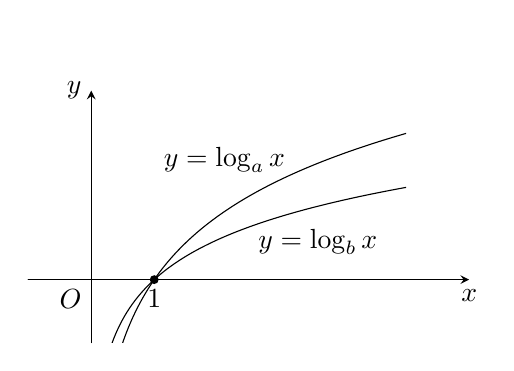
\begin{tikzpicture}[>=stealth,scale=0.8, line join=round, line cap=round]
			\draw[->] (-1,0)--(6,0) node [below]{$x$};
			\draw[->] (0,-1)--(0,3) node [left]{$y$};
			\node at (0,0) [below left]{$O$};
			\clip (-1,-1) rectangle (5,4);
			\fill[black] (1,0) circle (2pt) node [below] {$1$};
			\draw[smooth,samples=150,domain=0.1:5] plot(\x,{ln(\x)/ln(3)});
			\draw[smooth,samples=150,domain=0.1:5] plot(\x,{ln(\x)/ln(2)});
			\node at (2.5,0.6)[right]{$y=\log_b x$};
			\node at (1,1.9)[right]{$y=\log_a x$};
		\end{tikzpicture}
	}
	\loigiai{
		\immini{
			Quan sát đồ thị ta thấy cả hai đồ thị đều đi lên từ trái sang phải nên $a>1$ và $b>1$.\\
			Kẻ đường thẳng $y=1$ lần lượt cắt hai đồ thị $y=\log_a x$ và $y=\log_b x$ tại hai điểm $A(a;1); B(b;1)$. \\Nhìn vào đồ thị ta thấy  $a< b$.
		}
		{
			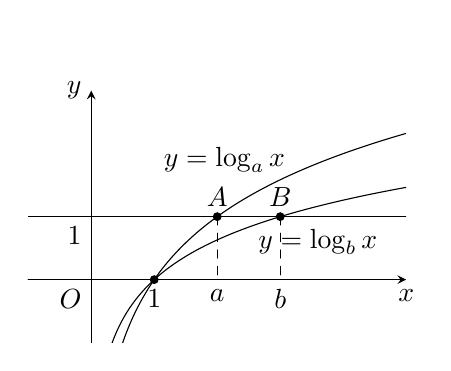
\begin{tikzpicture}[>=stealth,scale=0.8, line join=round, line cap=round]
				\draw[->] (-1,0)--(5,0) node [below]{$x$};
				\draw[->] (0,-1)--(0,3) node [left]{$y$};
				\node at (0,0) [below left]{$O$};
				\clip (-1,-1) rectangle (5,4);
				\draw  (-1,1)--(5,1) ;
				\fill[black] (1,0) circle (2pt) node [below] {$1$};
				\fill [black] (2,1) circle (2pt) node [above] {$A$};
				\fill [black] (3,1) circle (2pt) node [above] {$B$};
				\draw [dashed] (2,1)--(2,0) node [below] {$a$};
				\draw [dashed] (3,1)--(3,0) node [below] {$b$};
				\node at (0,1) [below left]{$1$};
				\draw[smooth,samples=150,domain=0.1:5] plot(\x,{ln(\x)/ln(3)});
				\draw[smooth,samples=150,domain=0.1:5] plot(\x,{ln(\x)/ln(2)});
				\node at (2.5,0.6)[right]{$y=\log_bx$};
				\node at (1,1.9)[right]{$y=\log_ax$};
			\end{tikzpicture}
		}
		
	}
\end{ex}

\begin{ex}%[Thành Đạt - Dự án Tex hoá tài liệu Dương Hùng]%[1D6H3-3]
	Giá trị của tham số $m$ để hàm số $y=\log_{(m+1)^2} x$ nghịch biến trên tập xác định của nó là
	\choice
	{$m \in(-\infty;0) \setminus\{-2;-1\}$}
	{$m \in(-\infty;0) \setminus\{-1\}$}
	{$m \in(-2;0)$}
	{\True $m \in(-2;0) \setminus\{-1\}$}
	\loigiai{
		Tập xác định $\mathscr{D}=(-1;+\infty)$.\\
		Hàm số nghịch biến trên $\mathscr{D}$ khi và chỉ khi\\
		$0<(m+1)^2<1 \Leftrightarrow \heva{&-1<m+1<1\\&m+1 \ne 0} \Leftrightarrow \heva{&-2<m<0 \\& m\ne-1.}$\\
		Vậy $m \in(-2;0) \setminus\{-1\}$ thì hàm số nghịch biến trên khoảng $(-1;+\infty)$.
	}
\end{ex}


\begin{ex}%[Thành Đạt - Dự án Tex hoá tài liệu Dương Hùng]%[1D6V3-3]
	\immini{ Cho $a,\,b,\,c$ là các số thực dương và khác $1$. Hình vẽ dưới đây là đồ thị của hàm số $y=\log_ax,\,y=\log_bx,\,y=\log_cx$. Khẳng định nào sau đây là đúng?
		\choice
		{$c<a<b$}
		{\True $b<c<a$}
		{$b<a<c$}
		{$a<b<c$}}
	{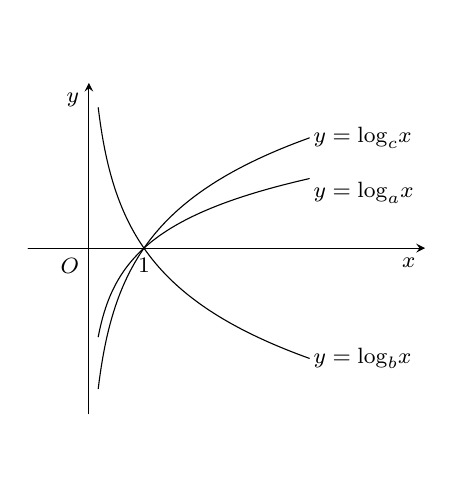
\begin{tikzpicture}[scale=0.7, font=\footnotesize, line join=round, line cap=round, >=stealth]
			\draw[->] (-1.1,0)--(6.1,0) node[below left] {$x$};
			\draw[->] (0,-3)--(0,3) node[below left] {$y$};
			\draw (0,0) node [below left] {$O$};
			\begin{scope}
				\clip (-1,-4) rectangle (5,4);
				\draw[samples=200,domain=0.17:4,smooth,variable=\x] plot (\x,{ln((\x))/ln(3)});
				\draw[samples=200,domain=0.17:4,smooth,variable=\x] plot (\x,{ln((\x))/ln(2)});
				\draw[samples=200,domain=0.17:4,smooth,variable=\x] plot (\x,{ln((\x))/ln(0.5)});
			\end{scope}
			\draw (3.9,-2) node[right]{$y={\log_{b}}x$};
			\draw (3.9,2) node[right]{$y={\log_{c}}x$};
			\draw (3.9,1) node[right]{$y={\log_{a}}x$};
			\draw (1,0)node[below]{$1$};
	\end{tikzpicture}}
	\loigiai{\immini{
			Ta vẽ thêm đường thẳng $y=1$ vào đồ thị đã cho.\\
			Nhận thấy rằng đường thẳng $y=1$ cắt 3 đồ thị $y=\log_ax,\,y=\log_bx,\,y=\log_cx$ lần lượt với $3$  giao điểm có hoành độ $x=a,\,x=b,\,x=c$.\\
			Dựa vào hình vẽ ta thấy $b<c<a$.	}{
			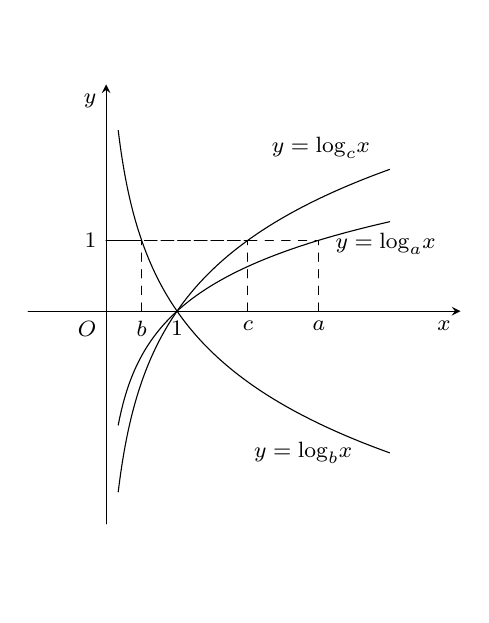
\begin{tikzpicture}[scale=0.9, font=\footnotesize, line join=round, line cap=round, >=stealth]
				\draw[->] (-1.1,0)--(5,0) node[below left] {$x$};
				\draw[->] (0,-3)--(0,3.2) node[below left] {$y$};
				\draw (0,0) node [below left] {$O$};
				\draw[dashed,thin](3,0)--(3,1)--(0,1);
				\draw[dashed,thin](2,0)--(2,1)--(0,1);
				\draw[dashed,thin](0.5,0)--(0.5,1)--(0,1);
				\begin{scope}
					\clip (-1,-4) rectangle (5,4);
					\draw[samples=200,domain=0.17:4,smooth,variable=\x] plot (\x,{ln((\x))/ln(3)});
					\draw[samples=200,domain=0.17:4,smooth,variable=\x] plot (\x,{ln((\x))/ln(2)});
					\draw[samples=200,domain=0.17:4,smooth,variable=\x] plot (\x,{ln((\x))/ln(0.5)});	
					\draw (1.95,-2) node[right]{$y={\log_{b}}x$};
					\draw (2.2,2.3) node[right]{$y={\log_{c}}x$};
					\draw (3.1,0.95) node[right]{$y={\log_{a}}x$};
					\draw (0,1)node[left]{$1$};
					\draw (1,0)node[below]{$1$};
					\draw (2,0)node[below]{$c$};
					\draw (3,0)node[below]{$a$};
					\draw (0.5,0)node[below]{$b$};
				\end{scope}
		\end{tikzpicture}}
	}
\end{ex}

\Closesolutionfile{ans}
\indapan{6}{ans/ans-K11-C6-B3-D2}
\cauds
\Opensolutionfile{ans}[ans/ans-K11-C6-B3-D2-DS]

\begin{ex}%[Thành Đạt - Dự án Tex hoá tài liệu Dương Hùng]%[1D6H3-2]
	Xét tập xác định của các hàm số.
	\choiceTF
%	[t]
	{\True Hàm số $y = \log_8 x$ có tập xác định là $\mathscr{D} = (0;+\infty)$}
	{\True Hàm số $y = \ln \dfrac{1}{x^2}$ có tập xác định là $\mathscr{D} = \mathbb{R}\setminus \{0\}$}
	{Hàm số $y=\mathrm{e}^{2x}$ có tập xác định là $\mathscr{D} = (0;+\infty)$}
	{Hàm số $y = \log x^2 + \log\dfrac{1}{x}$ có tập xác định là $\mathscr{D} = \mathbb{R}\setminus \{0\}$}
	\loigiai{
		\begin{itemchoice}
			\itemch \textbf{Đúng}.
			\itemch \textbf{Đúng}. Vì $\dfrac{1}{x^2} > 0 \Leftrightarrow x\ne 0$.
			\itemch \textbf{Sai}. Vì hàm số $y = \mathrm{e}^{2x}$ xác định trên $\mathbb{R}$.
			\itemch \textbf{Sai}. Vì $\heva{&x^2  > 0 \\ &\dfrac{1}{x} > 0} \Leftrightarrow x > 0$. 
		\end{itemchoice}	
	}
\end{ex}

\begin{ex}%[Thành Đạt - Dự án Tex hoá tài liệu Dương Hùng]%[1D6H3-4]
	Cho $a>1$.
	\choiceTF
%	[t]
	{\True $a^{6{,}3} > a^{6{,}2}$}
	{\True $\log_a (\sqrt{3} - 1) < \log_a (\sqrt{2} + 1)$}
	{$\log_a (\sqrt{3} - 2) < \log_a \sqrt{3}$}
	{$a^{3} < a^{2\sqrt{2}}$}
	\loigiai{
		Do $a > 1$ nên hàm số $y=a^x$ đồng biến trên $\mathbb{R}$ và hàm số $y=\log_a x$ đồng biến trên $(0;+\infty)$.
		\begin{itemchoice}
			\itemch \textbf{Đúng}. Vì $6{,}3 > 6{,}2$.
			\itemch \textbf{Đúng}. Vì $0 < \sqrt{3} - 1 <\sqrt{2} + 1$.
			\itemch \textbf{Sai}. Vì $\sqrt{3} - 2 < 0$.
			\itemch \textbf{Sai}. Vì $3 > 2\sqrt{2}$. 
		\end{itemchoice}	
	}
\end{ex}

\begin{ex}%[Thành Đạt - Dự án Tex hoá tài liệu Dương Hùng]
	Cho $a$ là số thực dương khác $1$.
	\choiceTF
%	[t]
	{Hàm số $y=\log_a x$ nghịch biến trên $(0;+\infty)$ khi $a>1$}
	{Hàm số $y=\log_a x$ có tập xác định là $\mathbb{R}$ khi $a<1$}
	{\True Hàm số $y=\log_a x$ có tập giá trị là $\mathbb{R}$}
	{\True Đồ thị của hàm số $y=\log_a x$ và $y=\log_{\tfrac{1}{a}} x$ (với $0<a<1$) đối xứng nhau qua trục hoành}
	\loigiai{
		\begin{itemchoice}
			\itemch \textbf{Sai}. 
			\itemch \textbf{Sai}.
			\itemch \textbf{Đúng}.
			\itemch\textbf{Đúng}.
		\end{itemchoice}	
	}
\end{ex}

\begin{ex}%[Thành Đạt - Dự án Tex hoá tài liệu Dương Hùng]%[1D6V3-3]
	\immini{
		Cho $a$, $b$, $c$ là các số thực dương và khác $1$. Hình bên là đồ thị của ba hàm số $y=a^{x}$, $y=b^{x}$, $y=c^{x}$ được vẽ trên một hệ trục tọa độ.}
	{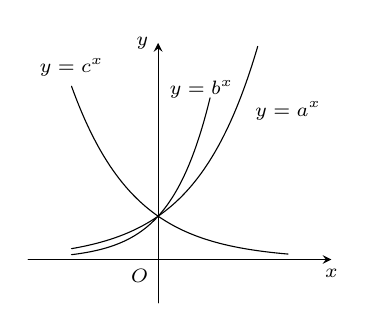
\begin{tikzpicture}[scale=0.55, font=\footnotesize, line join=round, line cap=round,>=stealth]
			\draw[->] (-3,0) -- (4,0) node[below] {\scriptsize $x$};
			\draw[->] (0,-1) -- (0,5) node[left] {\scriptsize $y$};
			\draw (0,0)node[below left]{\scriptsize $O$};
			\draw (3,3)node[above]{\scriptsize $ y=a^x $};
			\draw (1,3.5)node[above]{\scriptsize $ y=b^x $};
			\draw (-2,4)node[above]{\scriptsize $ y=c^x $};
			\draw[samples=150,smooth,domain=-2:2.3] plot(\x,{2^(\x)});
			\draw[samples=150,smooth,domain=-2:1.2] plot(\x,{3^(\x)});
			\draw[samples=150,smooth,domain=-2:3] plot(\x,{(0.5)^(\x)});
		\end{tikzpicture}
	}
	\choiceTF
%	[t]
	{\True $c^2 < 1$}
	{$a<1$}
	{$ab < 1$}
	{\True $a+b-c > 0$}
	\loigiai{
		Kẻ đường thẳng $ x=1 $ cắt đồ thị $ y=a^x $, $ y=b^x $ và $ y=c^x $ lần lượt tại các điểm $ A(1;a) $, $ B(1;b) $ và $ C(1;c) $.
		\begin{center}
			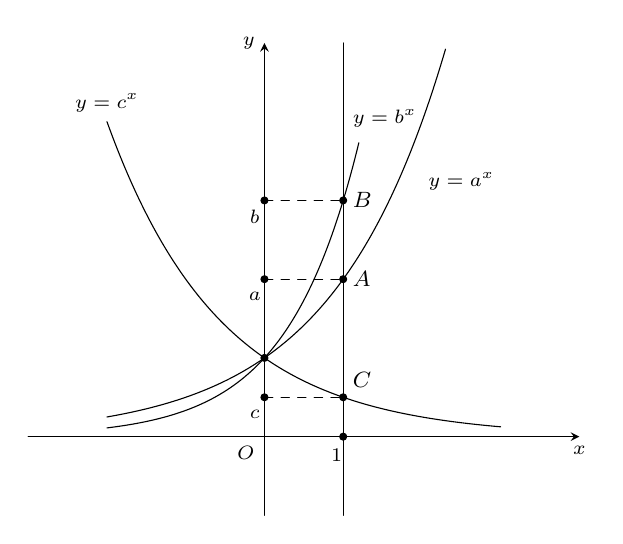
\begin{tikzpicture}[scale=1, font=\footnotesize, line join=round, line cap=round,>=stealth]
				\draw[->] (-3,0) -- (4,0) node[below] {\scriptsize $x$};
				\draw[->] (0,-1) -- (0,5) node[left] {\scriptsize $y$};
				\draw (0,0)node[below left]{\scriptsize $O$};
				\draw (2.5,3)node[above]{\scriptsize $ y=a^x $};
				\draw (1,3.8)node[above right]{\scriptsize $ y=b^x $};
				\draw (-2,4)node[above]{\scriptsize $ y=c^x $};
				\draw[samples=150,smooth,domain=-2:2.3] plot(\x,{2^(\x)});
				\draw[samples=150,smooth,domain=-2:1.2] plot(\x,{3^(\x)});
				\draw[samples=150,smooth,domain=-2:3] plot(\x,{(0.5)^(\x)});
				\draw[fill=black] (1,2) circle(1.25pt)node[right]{$ A $}
				(1,3) circle(1.25pt)node[right]{$ B $}
				(1,0.5) circle(1.25pt)node[above right]{$ C $}
				;
				\draw (1,-1)--(1,5);
				\draw[dashed] (0,0.5)--(1,0.5) (0,2)--(1,2) (0,3)--(1,3);
				\foreach \x/\y in{1/0,0/1/2,0/2,0/3,0/0.5}\draw[fill=black](\x,\y)circle(1.25pt);
				\foreach \x/\y/\goc/\z in{1/0/-110/1,0/0.5/-120/c,0/2/-120/a,0/3/-120/b}
				\path(\x,\y)node[shift={(\goc:7pt)}]{\scriptsize$\z$};
			\end{tikzpicture}
		\end{center}
		Dựa vào đồ thị, ta có hàm số $ y=c^x $ nghịch biến trên $ \mathbb{R} $ nên $ 0<c<1 $ và hàm số $ y=a^x $, $ y=b^x $ đồng biến trên $ \mathbb{R} $ nên $ 1<a$, $b$.\\
		Mặt khác $ y_A<y_B $ nên $ a<b $. Do đó $ 0<c<1<a<b $.
		\begin{itemchoice}
			\itemch \textbf{Đúng}. Vì $0 < c <1$ thì $c^2 < 1$.
			\itemch \textbf{Sai}.
			\itemch \textbf{Sai}. Vì $ab>1$
			\itemch\textbf{Đúng}. 
		\end{itemchoice}
	}
\end{ex}

\Closesolutionfile{ans}
\indapan{3}{ans/ans-K11-C6-B3-D2-DS}

\Opensolutionfile{ans}[ans/ans-K11-C6-B3-D2-KQ]
\caukq

\begin{ex}%[Thành Đạt - Dự án Tex hoá tài liệu Dương Hùng]%[1D6H3-3]
	Cho đồ thị của hàm số $y = 2^{ax+b}$ đi qua điểm $A(0;4)$ và $B(1;8)$. Tính giá trị $ab$.
	\shortans{$2$}
	\loigiai{
		Ta có $\heva{&2^b = 4\\ & 2^{a+b} = 8} \Leftrightarrow \heva{&b=2\\ &a+b=3} \Leftrightarrow \heva{&a=1\\ &b=2.}$\\
		Vậy $ab=2$.
	}
\end{ex}

\begin{ex}%[Thành Đạt - Dự án Tex hoá tài liệu Dương Hùng]%[1D6V3-3]
	\immini
	{
		Đồ thị trong hình vẽ dưới đây là đồ thị của hàm số $\log_a(bx+c)$ với $a$, $b$, $c$ là các số nguyên dương ($a\ne 1$). Biết tập xác định của hàm số là $(-1;+\infty)$, tính giá trị $a+b+c$.
		\shortans{$5$}
	}
	{
		\begin{tikzpicture}[>=stealth,scale=0.8, line join=round, line cap=round]
			\draw[->] (-2,0)--(3,0) node [below]{$x$};
			\draw[->] (0,-2)--(0,3) node [left]{$y$};
			\node at (0,0) [below right]{$O$};
			\clip (-2,-2) rectangle (3,3);
			\draw [dashed] (0,1) node [left]{$1$}--(2,1) --(2,0) node [below]{$2$};
			\draw[smooth,samples=150,domain=-0.9:3] plot(\x,{ln(\x +1)/ln(3)});
		\end{tikzpicture}
	}
	\loigiai{
		Ta có 
		\begin{itemize}
			\item Đồ thị của hàm số đi qua điểm $(0;0)$ nên $\log_a c = 0 \Leftrightarrow c =1$.
			\item Tập xác định của hàm số là $(-1;+\infty)$ nên bất phương trình $bx+1 > 0$ có tập nghiệm là $S = (-1;+\infty)$, điều này tương đương với 
			\[
			\heva{&b > 0\\ &\dfrac{-1}{b} = -1} \Leftrightarrow b =1.
			\] 
			\item Đồ thị của hàm số đi qua điểm $(2;1)$ nên $\log_a (1\cdot 2  +1) = 1 \Leftrightarrow \log_a 3 = 1 \Leftrightarrow a =3$.
		\end{itemize}
		Vậy $a+b+c = 5$.
	}
\end{ex}

\begin{ex}%[Thành Đạt - Dự án Tex hoá tài liệu Dương Hùng]%[1D6V3-2]
	Tập xác định của hàm số $y=\sqrt{\log_2\dfrac{2x}{1-x^2}}$ có dạng $[a;b)\cup[c;d)$. Tính giá trị của biểu thức $a+b+c+d$.
	\shortans{$-2$}
	\loigiai{
		Điều kiện: $ \heva{&\dfrac{2x}{1-x^2}>0\\&\log_2\dfrac{2x}{1-x^2}\ge 0}\Leftrightarrow \dfrac{2x}{1-x^2}\ge 1\Leftrightarrow \dfrac{x^2+2x-1}{1-x^2}\ge 0.$\\ 
		Đặt $T = \dfrac{x^2+2x-1}{1-x^2}$.\\
		Ta có 
		\begin{itemize}
			\item $x^2 + 2x - 1= 0 \Leftrightarrow \hoac{&x = x_1 = -1-\sqrt{2}\\ &x = x_2 = -1+\sqrt{2}.}$
			\item $1-x^2 = 0 \Leftrightarrow x = \pm 1$.
		\end{itemize}
		Khi đó ta có bảng xét dấu của $T$ như sau
		\begin{center}
			
\begin{tikzpicture}[line join=round, line cap = round, >=stealth, scale=.8,font=\footnotesize,transform shape]
				\tkzTabInit[nocadre=false,lgt=2.3,espcl=1.5,deltacl=0.6]
				{$x$ /1,
					$x^2 + 2x - 1$ /1,
					$1-x^2$ /1,
					$T$/1
				}% các hàng của bảng xét dấu
				{$-\infty$,$x_1$,$-1$,$x_2$,$1$,$+\infty$}
				\tkzTabLine { ,+,z,-,t,-,z,+,t,+, }
				\tkzTabLine { ,-,t,-,z,+,t,+,z,-, }
				\tkzTabLine { ,-,z,+,d,-,z,+,d,-, }
			\end{tikzpicture}
		\end{center}
		Dựa vào bảng xét dấu ta thấy $T \ge 0 \Leftrightarrow x\in \left[-1-\sqrt{2};-1\right)\cup\left[-1+\sqrt{2};1\right). $\\ 
		Suy ra $ a+b+c+d=-2. $
	}
\end{ex}

\begin{ex}%[Thành Đạt - Dự án Tex hoá tài liệu Dương Hùng]%[1D6V3-2]
	Tìm số số tự nhiên $m$ để hàm số $y=\dfrac{1}{\sqrt{2m+1-x}}+\log_3 \sqrt{x-m}$ xác định trên $(2;3)$.
	\shortans{$2$}
	\loigiai{
		Điều kiện để hàm số xác định là: $\heva{&2m+1-x>0 \\&x-m>0} \Leftrightarrow m<x<2m+1$.\\
		Hàm số xác định trên $(2;3)$ khi và chỉ khi $\heva{&m\le 2 \\&2m+1\ge 3} \Leftrightarrow 1\le m \le 2$. \\
		Vậy có $2$ số tự nhiên $m$ thoả mãn bài ra.
	}
\end{ex}

\begin{ex}%[Thành Đạt - Dự án Tex hoá tài liệu Dương Hùng]%[1D6V3-2]
	Tìm số giá trị nguyên của tham số m để hàm số $\log \left({{x}^{2}}-2mx+4 \right)$ có tập xác định $\mathbb{R}$.
	\shortans{$3$}
	\loigiai{
		Hàm số xác định trên $\mathbb{R}$ khi và chỉ khi
		$$x^2-2mx+4 >0, \, \forall x\in \mathbb{R} \Leftrightarrow \Delta'=m^2-4<0 \Leftrightarrow -2<m<2.$$
		Vậy có $3$ giá trị nguyên của $m$ thoả mãn.
	}
\end{ex}

\begin{ex}%[Thành Đạt - Dự án Tex hoá tài liệu Dương Hùng]%[1D6V3-3]
	\immini{Cho các hàm số $y=\log_a x$ và $y=\log_b x$ có đồ thị như hình vẽ bên. Đường thẳng $x=5$ cắt trục hoành, đồ thị hàm số $y=\log_a x$ và $y=\log_b x$ lần lượt tại $A$,  $B$ và $C$ . Biết rằng $CB=2AB$ và $a = mb^n$ với $m, n$ là các số nguyên dương. Tính $m^2 + n^2$.
		\shortans{$10$}
	}{
		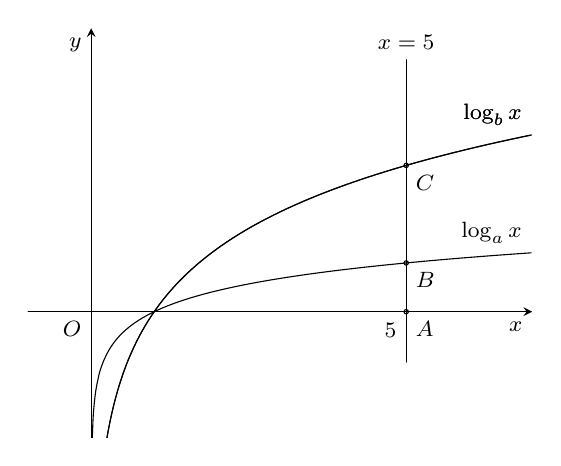
\begin{tikzpicture}[scale=0.8, font=\footnotesize, line join=round, line cap=round, >=stealth]
			\tikzset{label style/.style={font=\footnotesize}}
			
			\def \xmin{-1}
			\def \xmax{7}
			\def \ymin{-2}
			\def \ymax{4.5}
			\def \hamso{sin(\x r)}
			\draw[->] (\xmin,0)--(\xmax,0) node[below left] {$x$};
			\draw[->] (0,\ymin)--(0,\ymax) node[below left] {$y$};
			\draw (0,0) node [below left] {$O$};
			\foreach \x in {5}
			\draw[thin] (\x,1pt)--(\x,-1pt) node [below left] {$\x$};
			\begin{scope}
				\clip (\xmin+0.01,\ymin+0.01) rectangle (\xmax-0.01,\ymax-0.01);
				\draw[samples=350,domain=0.01:\xmax-0.01,smooth,variable=\x] plot (\x,{ln(\x)/ln(2)}) node[above left]{$\log_b x$};
				\draw[samples=350,domain=0.01:\xmax-0.01,smooth,variable=\x] plot (\x,{ln(\x)/ln(8)}) node[above left]{$\log_a x$};
				\draw[samples=350,domain=0.01:\xmax-0.01,smooth,variable=\x] plot (\x,{ln(\x)/ln(2)}) node[above left]{$\log_b x$};
				\draw(5,-0.8)--(5,4) node[above]{$x=5$};
				\draw(5.,0.) circle (1.0pt) node[below right]{$A$};
				\draw(5.,{ln(5)/ln(8)}) circle (1.0pt) node[below right]{$B$};
				\draw(5.,{ln(5)/ln(2)}) circle (1.0pt) node[below right]{$C$};
			\end{scope}
		\end{tikzpicture}
	}
	\loigiai
	{Ta có $A(5 ; 0)$, $B\left(5 ;\log_a5\right)$, $C\left(5 ;\log_b5\right)$. \\
		Do đó	
		\begin{eqnarray*}
			&CB=2AB &\Leftrightarrow\log_b5-\log_a5=2\log_a5\\
			&&\Leftrightarrow\log_b5=3\log_a5 \\
			&&\Leftrightarrow \log_5a=3\log_5b\\
			&&\Leftrightarrow a=b^3.
		\end{eqnarray*}
		Vậy $m=1$, $n=3$ nên $m^2 + n^2 = 10$.
	}
\end{ex}



\Closesolutionfile{ans}
\indapan{6}{ans/ans-K11-C6-B3-D2-KQ}